\documentclass[a4paper,14pt]{article}
\usepackage{float}
\usepackage{extsizes}
\usepackage{amsmath}
\usepackage{amssymb}
\everymath{\displaystyle}
\usepackage{geometry}
\usepackage{fancyhdr}
\usepackage{multicol}
\usepackage{graphicx}
\usepackage[brazil]{babel}
\usepackage[shortlabels]{enumitem}
\usepackage{cancel}
\usepackage{textcomp}
\usepackage{array}
\usepackage{longtable}
\usepackage{booktabs}
\usepackage{float}   % Para usar o modificador [H]

\columnsep=2cm
\hoffset=0cm
\textwidth=8cm
\setlength{\columnseprule}{.1pt}
\setlength{\columnsep}{2cm}
\renewcommand{\headrulewidth}{0pt}
\geometry{top=1in, bottom=1in, left=0.7in, right=0.5in}

\pagestyle{fancy}
\fancyhf{}
\fancyfoot[C]{\thepage}

\begin{document}
	
	\noindent\textbf{8FMA95 - Matemática} 
	
	\begin{center}Usando duas variáveis para resolver alguns problemas (IV) (Versão estudante)
	\end{center}
	
	\noindent\textbf{Nome:} \underline{\hspace{10cm}}
	\noindent\textbf{Data:} \underline{\hspace{4cm}}
	
	%\section*{Questões de Matemática}
    \begin{multicols}{2}
    	\begin{enumerate}
			\item Um zoológico abriga 3000 animais, entre terrestres, marinhos e aéreos. Sabendo que o dobro do número de animais aéreos somado ao número de animais marinhos é igual a 2000 e que o dobro do número de animais marinhos mais o número de animais aéreos é igual ao número de animais terrestres, determine a quantidade de cada tipo de animal do zoológico. \columnbreak
			\item Encontrar três números, sabendo-se que a soma deles é 31, que o triplo do primeiro mais o segundo é 30 e que três quintos do terceiro menos o segundo é 0. \newpage
			\item Para pesar três pacotes de massas distintas, dispomos de uma massa de 550 g e de uma balança de pratos iguais. A massa do pacote maior é igual ao dobro da massa dos outros dois juntos. A massa do menor mais 550 g iguala-se à massa dos outros dois juntos. O maior mais o menor têm, juntos, 600 g. Qual é a massa total dos três juntos? \columnbreak
			\item Complete o enunciado abaixo com os números dos quadros e, em seguida, resolva-o. Utilize um número do quadro I para a primeira lacuna e números do quadro II para a segunda e a terceira lacunas. \\
			Achar três números naturais distintos cuja soma é \underline{~~~~~~~~~~~~~~~~~~~~} e tais qua a razão entre o menor e o intermediário é \underline{~~~~~~~~~~~~~~~~} e entre o intermediário e o maior é \underline{~~~~~~~~~~~}.
			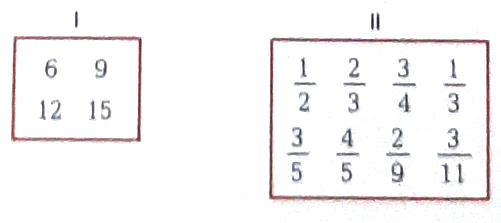
\includegraphics[width=1\linewidth]{imagens_8FMA95/imagem1}
			
			
    	\end{enumerate}
    $~$ \\ $~$ \\ $~$ \\ $~$ \\ $~$ \\ $~$ \\ $~$ \\ $~$ \\ $~$ \\ $~$ \\ $~$ \\ $~$ \\ $~$ \\ $~$ \\ $~$ \\ $~$ \\ $~$ \\ $~$ \\ $~$ \\ $~$ \\ $~$ \\ $~$ \\
    \end{multicols}
\end{document}